\subsection{Sender Side (RTC Transmission Pipeline)}

The sender-side is responsible for transforming a speaker's voice into a compressed network stream suitable for real-time communication. In the proposed framework, the sender-side pipeline is treated as a standard RTC subsystem and is not modified by the detection mechanism and serves as a realistic source of audio data that reflects practical deployment conditions found in VoIP and conferencing systems.

\begin{figure}[H]
    \centering
    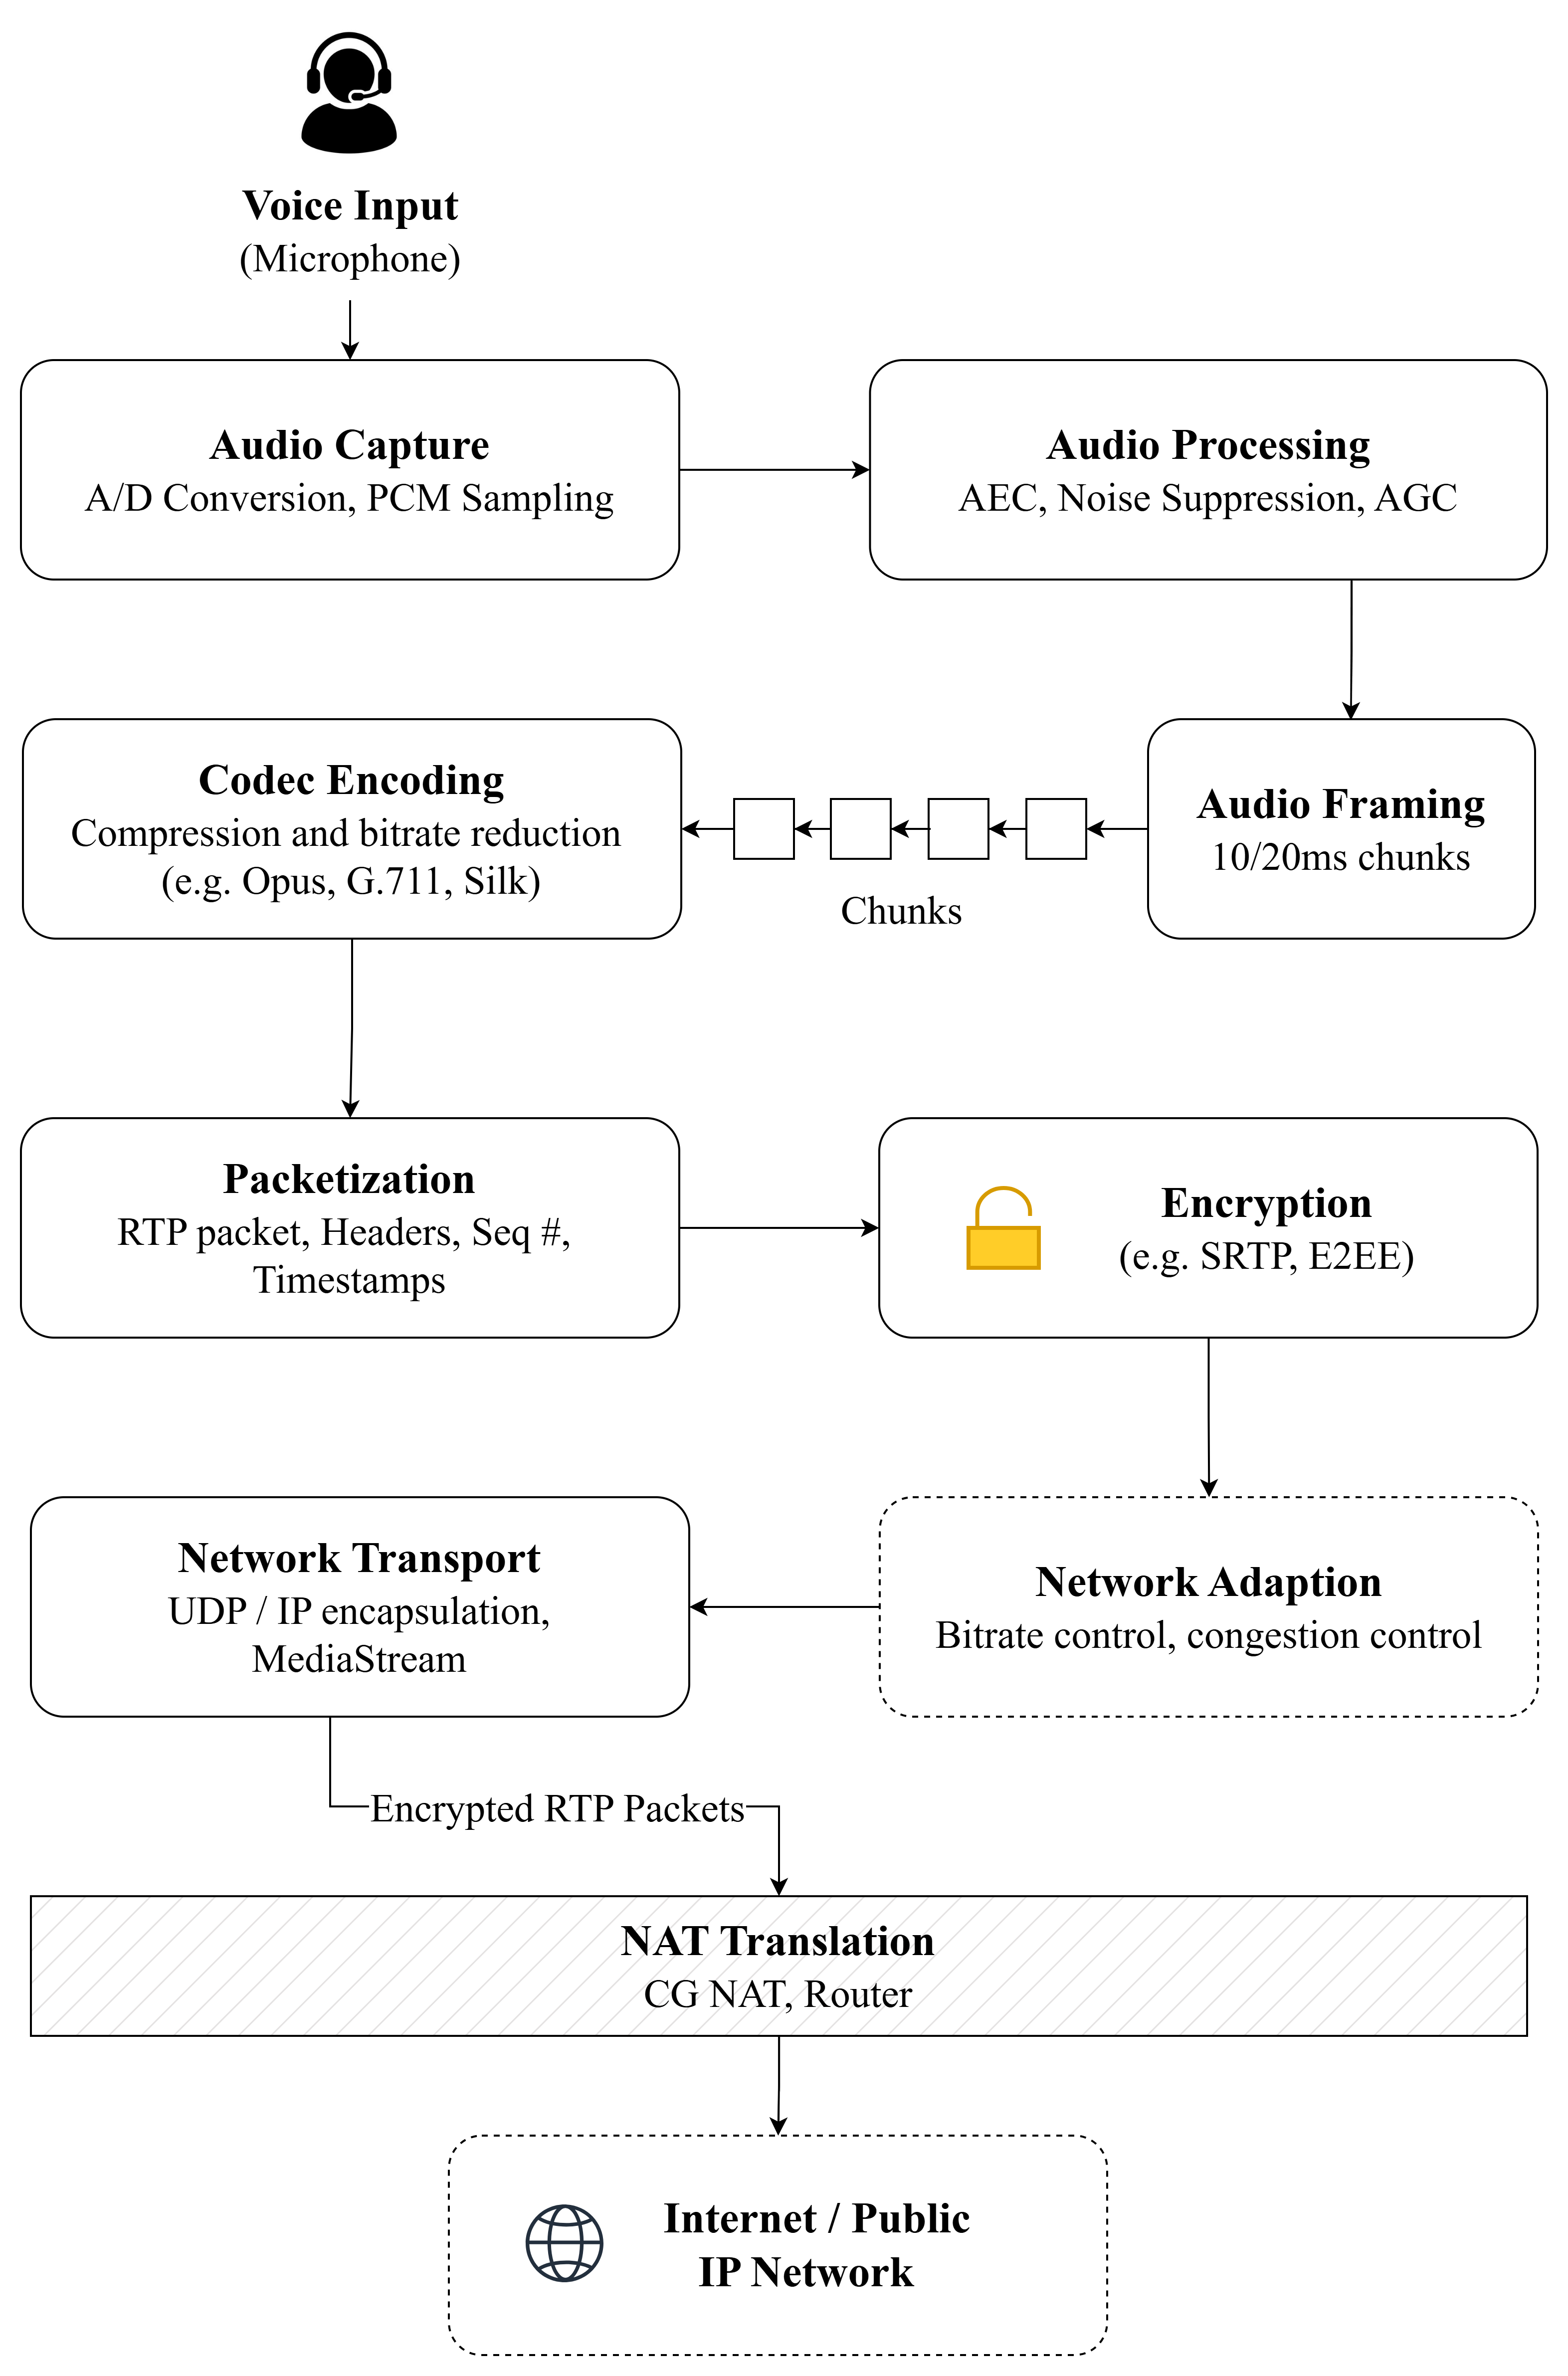
\includegraphics[width=1\textwidth]{images/methodology/sender_side.png}
    \vspace{0.25cm}
    \caption{Sender-side RTC Transmission Pipeline}
    \label{fig:sender_side}
\end{figure}


\subsubsection{Audio Capture and Pre-processing}

The transmission process begins with acquisition of speech through a microphone device. The analog speech waveform is converted into a digital signal through Analog-to-Digital Conversion (ADC), where sampling and quantization are performed at a predefined sampling rate (typically ranging from 16 kHz to 48 kHz).

Let the continuous-time speech signal be represented as $x(t)$ which is transformed into a discrete-time representation $x[n]$ through the sampling process.

Depending on the operating system and device capabilities, additional preprocessing may be applied, including acoustic echo cancellation, noise suppression, and gain normalization. These operations improve speech intelligibility but may also alter spectral characteristics relevant to deepfake analysis.

Here, the signal remains in a near-natural form but may already include environmental noise and recording artifacts. This stage introduces uncontrolled variability (speaker device, environment), which contributes to domain diversity in downstream detection.

\subsubsection{Audio Framing}

The processed audio stream is divided into small fixed duration frames, typically ranging from 10ms to 20ms. Framing allows the system to process and transmit audio incrementally rather than waiting for larger audio segments. 

Each frame serves as an independent unit for encoding and network transmission.

\subsubsection{Encoding and Compression}

The preprocessed audio signal is compressed using a speech codec before transmission. Modern RTC systems typically employ codecs such as Opus due to their low latency and adaptive bitrate capabilities. 

Let $x[n]$ denote the input waveform and $C(\cdot)$ denote the codec transformation:
\begin{equation}
x_c = C(x[n])
\label{eq:codec_transform}
\end{equation}
where $x_c$ is the compressed bitstream representation.

Compression reduces transmission bandwidth requirements but introduces codec-specific distortions, including quantization noise, spectral smoothing, and loss of fine-grained acoustic information. These effects may partially mask or modify artifacts generated by synthetic speech systems.

\subsubsection{Packetization}

The compressed audio stream is segmented into small packets suitable for real-time delivery. Each packet is encapsulated into transport packets containing timing and synchronization metadata.

The packetization process is represented as
\begin{equation}
x_c \rightarrow \{p_1, p_2, \ldots, p_n\}
\label{eq:packetization}
\end{equation}
where $p_i$ represents an individual network packet.

Each packet generally contains a compressed payload along with sequence numbers and timestamps required for stream reconstruction at the receiver.

\subsubsection{Encryption and Security}

To ensure confidentiality and protect user privacy, voice packets are encrypted before transmission. The proposed system employs end-to-end encryption (E2EE), ensuring that only the communicating participants can access the contents of the conversation. Even if network traffic is intercepted, unauthorized parties cannot recover the original audio data without the corresponding cryptographic keys.

During call establishment, a secure key exchange mechanism is performed between the communicating parties. Modern public-key cryptographic algorithms such as X25519 (Elliptic Curve Diffie–Hellman) are used to derive a shared session key without transmitting the key itself over the network. 

Once a secure session key has been established, the audio stream is encrypted using a symmetric encryption algorithm such as AES-256-GCM or ChaCha20-Poly1305. These algorithms provide both confidentiality and integrity protection for transmitted audio packets.

The encrypted audio packets are then encapsulated using the Secure Real-Time Transport Protocol (SRTP), which provides secure delivery of real-time voice data. Finally, the packets are transmitted over UDP, a low-latency transport protocol commonly used in real-time communication systems due to its minimal transmission overhead and reduced delay characteristics.

\subsubsection{Network Transport}

Following encryption, the protected audio packets are prepared for network transmission. The encrypted SRTP packet is encapsulated within a UDP datagram, which provides a lightweight and low-latency transport mechanism suitable for real-time communication.

The UDP datagram is subsequently encapsulated within an IP packet containing the source and destination addressing information required for routing across the network. This layered encapsulation enables intermediate networking devices to forward packets toward the intended recipient.

Once packet construction is complete, the operating system transmits the packet through the available network interface, such as Wi-Fi or cellular data. The sender continuously generates, encrypts, encapsulates, and transmits packets throughout the duration of the call, forming a secure real-time voice stream between communicating users.